% Created by tikzDevice version 0.12.6 on 2025-05-12 11:29:26
% !TEX encoding = UTF-8 Unicode
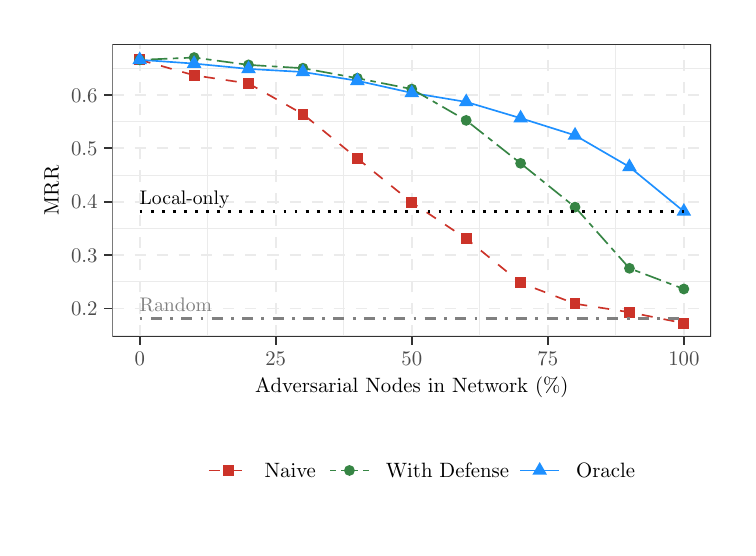
\begin{tikzpicture}[x=1pt,y=1pt]
\definecolor{fillColor}{RGB}{255,255,255}
\path[use as bounding box,fill=fillColor,fill opacity=0.00] (0,0) rectangle (252.94,180.67);
\begin{scope}
\path[clip] (  0.00,  0.00) rectangle (252.94,180.67);
\definecolor{drawColor}{RGB}{255,255,255}
\definecolor{fillColor}{RGB}{255,255,255}

\path[draw=drawColor,line width= 0.6pt,line join=round,line cap=round,fill=fillColor] (  0.00, -0.00) rectangle (252.94,180.67);
\end{scope}
\begin{scope}
\path[clip] ( 30.65, 69.07) rectangle (246.95,174.67);
\definecolor{fillColor}{RGB}{255,255,255}

\path[fill=fillColor] ( 30.65, 69.07) rectangle (246.95,174.67);
\definecolor{drawColor}{gray}{0.92}

\path[draw=drawColor,line width= 0.3pt,line join=round] ( 30.65, 69.49) --
	(246.95, 69.49);

\path[draw=drawColor,line width= 0.3pt,line join=round] ( 30.65, 88.80) --
	(246.95, 88.80);

\path[draw=drawColor,line width= 0.3pt,line join=round] ( 30.65,108.11) --
	(246.95,108.11);

\path[draw=drawColor,line width= 0.3pt,line join=round] ( 30.65,127.42) --
	(246.95,127.42);

\path[draw=drawColor,line width= 0.3pt,line join=round] ( 30.65,146.73) --
	(246.95,146.73);

\path[draw=drawColor,line width= 0.3pt,line join=round] ( 30.65,166.04) --
	(246.95,166.04);

\path[draw=drawColor,line width= 0.3pt,line join=round] ( 65.06, 69.07) --
	( 65.06,174.67);

\path[draw=drawColor,line width= 0.3pt,line join=round] (114.22, 69.07) --
	(114.22,174.67);

\path[draw=drawColor,line width= 0.3pt,line join=round] (163.37, 69.07) --
	(163.37,174.67);

\path[draw=drawColor,line width= 0.3pt,line join=round] (212.53, 69.07) --
	(212.53,174.67);

\path[draw=drawColor,line width= 0.6pt,dash pattern=on 4pt off 4pt ,line join=round] ( 30.65, 79.14) --
	(246.95, 79.14);

\path[draw=drawColor,line width= 0.6pt,dash pattern=on 4pt off 4pt ,line join=round] ( 30.65, 98.46) --
	(246.95, 98.46);

\path[draw=drawColor,line width= 0.6pt,dash pattern=on 4pt off 4pt ,line join=round] ( 30.65,117.77) --
	(246.95,117.77);

\path[draw=drawColor,line width= 0.6pt,dash pattern=on 4pt off 4pt ,line join=round] ( 30.65,137.08) --
	(246.95,137.08);

\path[draw=drawColor,line width= 0.6pt,dash pattern=on 4pt off 4pt ,line join=round] ( 30.65,156.39) --
	(246.95,156.39);

\path[draw=drawColor,line width= 0.6pt,dash pattern=on 4pt off 4pt ,line join=round] ( 40.48, 69.07) --
	( 40.48,174.67);

\path[draw=drawColor,line width= 0.6pt,dash pattern=on 4pt off 4pt ,line join=round] ( 89.64, 69.07) --
	( 89.64,174.67);

\path[draw=drawColor,line width= 0.6pt,dash pattern=on 4pt off 4pt ,line join=round] (138.80, 69.07) --
	(138.80,174.67);

\path[draw=drawColor,line width= 0.6pt,dash pattern=on 4pt off 4pt ,line join=round] (187.95, 69.07) --
	(187.95,174.67);

\path[draw=drawColor,line width= 0.6pt,dash pattern=on 4pt off 4pt ,line join=round] (237.11, 69.07) --
	(237.11,174.67);
\definecolor{drawColor}{RGB}{204,51,41}

\path[draw=drawColor,line width= 0.6pt,dash pattern=on 4pt off 4pt ,line join=round] ( 40.48,169.06) --
	( 60.14,163.46) --
	( 79.80,160.51) --
	( 99.47,149.42) --
	(119.13,133.41) --
	(138.80,117.51) --
	(158.46,104.43) --
	(178.12, 88.48) --
	(197.79, 80.91) --
	(217.45, 77.85) --
	(237.11, 73.87);
\definecolor{drawColor}{RGB}{30,144,255}

\path[draw=drawColor,line width= 0.6pt,line join=round] ( 40.48,169.06) --
	( 60.14,167.69) --
	( 79.80,165.77) --
	( 99.47,164.65) --
	(119.13,161.48) --
	(138.80,157.10) --
	(158.46,153.84) --
	(178.12,147.97) --
	(197.79,141.77) --
	(217.45,130.36) --
	(237.11,114.26);
\definecolor{drawColor}{RGB}{54,133,68}

\path[draw=drawColor,line width= 0.6pt,dash pattern=on 2pt off 2pt on 6pt off 2pt ,line join=round] ( 40.48,169.04) --
	( 60.14,169.87) --
	( 79.80,167.22) --
	( 99.47,166.02) --
	(119.13,162.41) --
	(138.80,158.48) --
	(158.46,147.16) --
	(178.12,131.65) --
	(197.79,115.82) --
	(217.45, 93.71) --
	(237.11, 86.24);
\definecolor{fillColor}{RGB}{204,51,41}

\path[fill=fillColor] ( 38.52,167.09) --
	( 42.44,167.09) --
	( 42.44,171.02) --
	( 38.52,171.02) --
	cycle;
\definecolor{fillColor}{RGB}{54,133,68}

\path[fill=fillColor] ( 40.48,169.04) circle (  1.96);
\definecolor{fillColor}{RGB}{30,144,255}

\path[fill=fillColor] ( 40.48,172.11) --
	( 43.12,167.53) --
	( 37.84,167.53) --
	cycle;
\definecolor{fillColor}{RGB}{204,51,41}

\path[fill=fillColor] ( 58.18,161.50) --
	( 62.10,161.50) --
	( 62.10,165.42) --
	( 58.18,165.42) --
	cycle;
\definecolor{fillColor}{RGB}{54,133,68}

\path[fill=fillColor] ( 60.14,169.87) circle (  1.96);
\definecolor{fillColor}{RGB}{30,144,255}

\path[fill=fillColor] ( 60.14,170.74) --
	( 62.78,166.16) --
	( 57.50,166.16) --
	cycle;
\definecolor{fillColor}{RGB}{204,51,41}

\path[fill=fillColor] ( 77.84,158.55) --
	( 81.77,158.55) --
	( 81.77,162.47) --
	( 77.84,162.47) --
	cycle;
\definecolor{fillColor}{RGB}{54,133,68}

\path[fill=fillColor] ( 79.80,167.22) circle (  1.96);
\definecolor{fillColor}{RGB}{30,144,255}

\path[fill=fillColor] ( 79.80,168.82) --
	( 82.45,164.24) --
	( 77.16,164.24) --
	cycle;
\definecolor{fillColor}{RGB}{204,51,41}

\path[fill=fillColor] ( 97.51,147.45) --
	(101.43,147.45) --
	(101.43,151.38) --
	( 97.51,151.38) --
	cycle;
\definecolor{fillColor}{RGB}{54,133,68}

\path[fill=fillColor] ( 99.47,166.02) circle (  1.96);
\definecolor{fillColor}{RGB}{30,144,255}

\path[fill=fillColor] ( 99.47,167.70) --
	(102.11,163.13) --
	( 96.83,163.13) --
	cycle;
\definecolor{fillColor}{RGB}{204,51,41}

\path[fill=fillColor] (117.17,131.45) --
	(121.09,131.45) --
	(121.09,135.38) --
	(117.17,135.38) --
	cycle;
\definecolor{fillColor}{RGB}{54,133,68}

\path[fill=fillColor] (119.13,162.41) circle (  1.96);
\definecolor{fillColor}{RGB}{30,144,255}

\path[fill=fillColor] (119.13,164.53) --
	(121.77,159.95) --
	(116.49,159.95) --
	cycle;
\definecolor{fillColor}{RGB}{204,51,41}

\path[fill=fillColor] (136.83,115.55) --
	(140.76,115.55) --
	(140.76,119.48) --
	(136.83,119.48) --
	cycle;
\definecolor{fillColor}{RGB}{54,133,68}

\path[fill=fillColor] (138.80,158.48) circle (  1.96);
\definecolor{fillColor}{RGB}{30,144,255}

\path[fill=fillColor] (138.80,160.15) --
	(141.44,155.58) --
	(136.15,155.58) --
	cycle;
\definecolor{fillColor}{RGB}{204,51,41}

\path[fill=fillColor] (156.50,102.47) --
	(160.42,102.47) --
	(160.42,106.39) --
	(156.50,106.39) --
	cycle;
\definecolor{fillColor}{RGB}{54,133,68}

\path[fill=fillColor] (158.46,147.16) circle (  1.96);
\definecolor{fillColor}{RGB}{30,144,255}

\path[fill=fillColor] (158.46,156.89) --
	(161.10,152.31) --
	(155.82,152.31) --
	cycle;
\definecolor{fillColor}{RGB}{204,51,41}

\path[fill=fillColor] (176.16, 86.51) --
	(180.08, 86.51) --
	(180.08, 90.44) --
	(176.16, 90.44) --
	cycle;
\definecolor{fillColor}{RGB}{54,133,68}

\path[fill=fillColor] (178.12,131.65) circle (  1.96);
\definecolor{fillColor}{RGB}{30,144,255}

\path[fill=fillColor] (178.12,151.02) --
	(180.77,146.45) --
	(175.48,146.45) --
	cycle;
\definecolor{fillColor}{RGB}{204,51,41}

\path[fill=fillColor] (195.82, 78.94) --
	(199.75, 78.94) --
	(199.75, 82.87) --
	(195.82, 82.87) --
	cycle;
\definecolor{fillColor}{RGB}{54,133,68}

\path[fill=fillColor] (197.79,115.82) circle (  1.96);
\definecolor{fillColor}{RGB}{30,144,255}

\path[fill=fillColor] (197.79,144.82) --
	(200.43,140.24) --
	(195.14,140.24) --
	cycle;
\definecolor{fillColor}{RGB}{204,51,41}

\path[fill=fillColor] (215.49, 75.89) --
	(219.41, 75.89) --
	(219.41, 79.81) --
	(215.49, 79.81) --
	cycle;
\definecolor{fillColor}{RGB}{54,133,68}

\path[fill=fillColor] (217.45, 93.71) circle (  1.96);
\definecolor{fillColor}{RGB}{30,144,255}

\path[fill=fillColor] (217.45,133.41) --
	(220.09,128.83) --
	(214.81,128.83) --
	cycle;
\definecolor{fillColor}{RGB}{204,51,41}

\path[fill=fillColor] (235.15, 71.91) --
	(239.08, 71.91) --
	(239.08, 75.84) --
	(235.15, 75.84) --
	cycle;
\definecolor{fillColor}{RGB}{54,133,68}

\path[fill=fillColor] (237.11, 86.24) circle (  1.96);
\definecolor{fillColor}{RGB}{30,144,255}

\path[fill=fillColor] (237.11,117.31) --
	(239.76,112.74) --
	(234.47,112.74) --
	cycle;
\definecolor{drawColor}{RGB}{0,0,0}

\path[draw=drawColor,line width= 1.1pt,dash pattern=on 1pt off 3pt ,line join=round] ( 40.48,114.26) --
	(237.11,114.26);
\definecolor{drawColor}{gray}{0.50}

\path[draw=drawColor,line width= 1.1pt,dash pattern=on 1pt off 3pt on 4pt off 3pt ,line join=round] ( 40.48, 75.63) --
	(237.11, 75.63);
\definecolor{drawColor}{RGB}{0,0,0}

\node[text=drawColor,anchor=base west,inner sep=0pt, outer sep=0pt, scale=  0.71] at ( 40.48,116.73) {Local-only};
\definecolor{drawColor}{gray}{0.50}

\node[text=drawColor,anchor=base west,inner sep=0pt, outer sep=0pt, scale=  0.71] at ( 40.48, 78.10) {Random};
\definecolor{drawColor}{gray}{0.20}

\path[draw=drawColor,line width= 0.6pt,line join=round,line cap=round] ( 30.65, 69.07) rectangle (246.95,174.67);
\end{scope}
\begin{scope}
\path[clip] (  0.00,  0.00) rectangle (252.94,180.67);
\definecolor{drawColor}{gray}{0.30}

\node[text=drawColor,anchor=base east,inner sep=0pt, outer sep=0pt, scale=  0.75] at ( 25.25, 76.54) {0.2};

\node[text=drawColor,anchor=base east,inner sep=0pt, outer sep=0pt, scale=  0.75] at ( 25.25, 95.85) {0.3};

\node[text=drawColor,anchor=base east,inner sep=0pt, outer sep=0pt, scale=  0.75] at ( 25.25,115.16) {0.4};

\node[text=drawColor,anchor=base east,inner sep=0pt, outer sep=0pt, scale=  0.75] at ( 25.25,134.47) {0.5};

\node[text=drawColor,anchor=base east,inner sep=0pt, outer sep=0pt, scale=  0.75] at ( 25.25,153.78) {0.6};
\end{scope}
\begin{scope}
\path[clip] (  0.00,  0.00) rectangle (252.94,180.67);
\definecolor{drawColor}{gray}{0.20}

\path[draw=drawColor,line width= 0.6pt,line join=round] ( 27.65, 79.14) --
	( 30.65, 79.14);

\path[draw=drawColor,line width= 0.6pt,line join=round] ( 27.65, 98.46) --
	( 30.65, 98.46);

\path[draw=drawColor,line width= 0.6pt,line join=round] ( 27.65,117.77) --
	( 30.65,117.77);

\path[draw=drawColor,line width= 0.6pt,line join=round] ( 27.65,137.08) --
	( 30.65,137.08);

\path[draw=drawColor,line width= 0.6pt,line join=round] ( 27.65,156.39) --
	( 30.65,156.39);
\end{scope}
\begin{scope}
\path[clip] (  0.00,  0.00) rectangle (252.94,180.67);
\definecolor{drawColor}{gray}{0.20}

\path[draw=drawColor,line width= 0.6pt,line join=round] ( 40.48, 66.07) --
	( 40.48, 69.07);

\path[draw=drawColor,line width= 0.6pt,line join=round] ( 89.64, 66.07) --
	( 89.64, 69.07);

\path[draw=drawColor,line width= 0.6pt,line join=round] (138.80, 66.07) --
	(138.80, 69.07);

\path[draw=drawColor,line width= 0.6pt,line join=round] (187.95, 66.07) --
	(187.95, 69.07);

\path[draw=drawColor,line width= 0.6pt,line join=round] (237.11, 66.07) --
	(237.11, 69.07);
\end{scope}
\begin{scope}
\path[clip] (  0.00,  0.00) rectangle (252.94,180.67);
\definecolor{drawColor}{gray}{0.30}

\node[text=drawColor,anchor=base,inner sep=0pt, outer sep=0pt, scale=  0.75] at ( 40.48, 58.47) {0};

\node[text=drawColor,anchor=base,inner sep=0pt, outer sep=0pt, scale=  0.75] at ( 89.64, 58.47) {25};

\node[text=drawColor,anchor=base,inner sep=0pt, outer sep=0pt, scale=  0.75] at (138.80, 58.47) {50};

\node[text=drawColor,anchor=base,inner sep=0pt, outer sep=0pt, scale=  0.75] at (187.95, 58.47) {75};

\node[text=drawColor,anchor=base,inner sep=0pt, outer sep=0pt, scale=  0.75] at (237.11, 58.47) {100};
\end{scope}
\begin{scope}
\path[clip] (  0.00,  0.00) rectangle (252.94,180.67);
\definecolor{drawColor}{RGB}{0,0,0}

\node[text=drawColor,anchor=base,inner sep=0pt, outer sep=0pt, scale=  0.75] at (138.80, 48.80) {Adversarial Nodes in Network ({\%})};
\end{scope}
\begin{scope}
\path[clip] (  0.00,  0.00) rectangle (252.94,180.67);
\definecolor{drawColor}{RGB}{0,0,0}

\node[text=drawColor,rotate= 90.00,anchor=base,inner sep=0pt, outer sep=0pt, scale=  0.75] at ( 11.21,121.87) {MRR};
\end{scope}
\begin{scope}
\path[clip] (  0.00,  0.00) rectangle (252.94,180.67);
\definecolor{fillColor}{RGB}{255,255,255}

\path[fill=fillColor] ( 53.26,  6.00) rectangle (224.33, 35.34);
\end{scope}
\begin{scope}
\path[clip] (  0.00,  0.00) rectangle (252.94,180.67);
\definecolor{fillColor}{RGB}{255,255,255}

\path[fill=fillColor] ( 63.76, 12.00) rectangle ( 81.10, 29.34);
\end{scope}
\begin{scope}
\path[clip] (  0.00,  0.00) rectangle (252.94,180.67);
\definecolor{drawColor}{RGB}{204,51,41}

\path[draw=drawColor,line width= 0.6pt,dash pattern=on 4pt off 4pt ,line join=round] ( 65.49, 20.67) -- ( 79.37, 20.67);
\end{scope}
\begin{scope}
\path[clip] (  0.00,  0.00) rectangle (252.94,180.67);
\definecolor{fillColor}{RGB}{204,51,41}

\path[fill=fillColor] ( 70.47, 18.71) --
	( 74.39, 18.71) --
	( 74.39, 22.63) --
	( 70.47, 22.63) --
	cycle;
\end{scope}
\begin{scope}
\path[clip] (  0.00,  0.00) rectangle (252.94,180.67);
\definecolor{fillColor}{RGB}{255,255,255}

\path[fill=fillColor] (107.60, 12.00) rectangle (124.94, 29.34);
\end{scope}
\begin{scope}
\path[clip] (  0.00,  0.00) rectangle (252.94,180.67);
\definecolor{drawColor}{RGB}{54,133,68}

\path[draw=drawColor,line width= 0.6pt,dash pattern=on 2pt off 2pt on 6pt off 2pt ,line join=round] (109.33, 20.67) -- (123.21, 20.67);
\end{scope}
\begin{scope}
\path[clip] (  0.00,  0.00) rectangle (252.94,180.67);
\definecolor{fillColor}{RGB}{54,133,68}

\path[fill=fillColor] (116.27, 20.67) circle (  1.96);
\end{scope}
\begin{scope}
\path[clip] (  0.00,  0.00) rectangle (252.94,180.67);
\definecolor{fillColor}{RGB}{255,255,255}

\path[fill=fillColor] (176.35, 12.00) rectangle (193.69, 29.34);
\end{scope}
\begin{scope}
\path[clip] (  0.00,  0.00) rectangle (252.94,180.67);
\definecolor{drawColor}{RGB}{30,144,255}

\path[draw=drawColor,line width= 0.6pt,line join=round] (178.08, 20.67) -- (191.96, 20.67);
\end{scope}
\begin{scope}
\path[clip] (  0.00,  0.00) rectangle (252.94,180.67);
\definecolor{fillColor}{RGB}{30,144,255}

\path[fill=fillColor] (185.02, 23.72) --
	(187.66, 19.15) --
	(182.38, 19.15) --
	cycle;
\end{scope}
\begin{scope}
\path[clip] (  0.00,  0.00) rectangle (252.94,180.67);
\definecolor{drawColor}{RGB}{0,0,0}

\node[text=drawColor,anchor=base west,inner sep=0pt, outer sep=0pt, scale=  0.75] at ( 85.60, 18.07) {Naive};
\end{scope}
\begin{scope}
\path[clip] (  0.00,  0.00) rectangle (252.94,180.67);
\definecolor{drawColor}{RGB}{0,0,0}

\node[text=drawColor,anchor=base west,inner sep=0pt, outer sep=0pt, scale=  0.75] at (129.44, 18.07) {With Defense};
\end{scope}
\begin{scope}
\path[clip] (  0.00,  0.00) rectangle (252.94,180.67);
\definecolor{drawColor}{RGB}{0,0,0}

\node[text=drawColor,anchor=base west,inner sep=0pt, outer sep=0pt, scale=  0.75] at (198.19, 18.07) {Oracle};
\end{scope}
\end{tikzpicture}
